
\documentclass[10pt,a4paper,titlepage]{report}
\usepackage[utf8]{inputenc}
\usepackage{amsmath}
\usepackage{amsfonts}
\usepackage{amssymb}
\usepackage{graphicx}
\usepackage{xcolor}
\usepackage{minted}
\usepackage{geometry}
\geometry{
	left=4cm
}
\usepackage[hidelinks]{hyperref}
\usepackage{fancyhdr}
 \usemintedstyle{xcode}
\pagestyle{fancy}
\fancyhf{}
\cfoot{\thepage}
\renewcommand{\headrulewidth}{0.01cm}

\newcommand{\HRule}[1]{\rule{\linewidth}{#1}}
\renewcommand{\chaptername}{Experiment}

\nonstopmode


\begin{document}
% \begin{titlepage}

% \begin{center}
% {\LARGE College Of Engineering, Trivandrum}\\[1cm]
% \linespread{1.2}\huge {\bfseries Application Software Development Lab\\CS333}\\[1cm]
% \linespread{1}
% 
\includegraphics[width=5cm]{../Images/index.jpeg}\\[1cm]
% {\Large Rwithik Manoj\\ S5  CSE Roll No:53\\ TVE17CS054 }\\[1cm]
% {\large \emph{Supervisors:} Vipin Vasu A V , Remya Krishnan}\\ [0.7cm]% if applicable
% \large A report submitted in partial fulfilment of ASD lab work \\in Semester 5\\[0.3cm] 
% \textit{in the}\\[0.3cm]
% Department of Computer Science\\[0.5cm]
% \today
% \end{center}

% \end{titlepage}

\begin{titlepage}
\vfill
\begin{center}

\includegraphics[width=2cm]{../Images/index.jpeg}
\\[1cm]
\begin{LARGE}
\uppercase{College of Engineering}
\\[0.3cm]
\uppercase{Trivandrum}
\end{LARGE}
\\[1.5cm]
\uppercase{Computer science and engineering}
\\[0.2cm]
\uppercase{Application software development lab}
\\[0.5cm]
{\Large CSE 333}
\\[1cm]
{\Large\uppercase{Application software development lab \\[0.1cm] report}}
\HRule{0.01cm}
\\[0.5cm]
\uppercase{Certified bonafide record of work done by}
\\[0.5cm]
\uppercase{Rwithik Manoj}
\\[0.4cm]
\textsc{University Reg. No: TVE17CS054}
\\[0.4cm]
\textsc{Roll No: 53}
\\[0.4cm]
\textsc{Class: S5 CSE}
\end{center}
\vfill
\textsc{Staff In-charge:}\\[0.4cm]
VIPIN VASU A.V, REMYA KRISHNAN\\[0.4cm]
\textsc{Department of Computer Science and Engineering}
\end{titlepage}

% \maketitle
\tableofcontents
\newpage

\sectionfont{\scshape}
\chapterfont{\scshape}

\chapter{Installation of POSTGRESQL}
\documentclass[10pt,a4paper,titlepage]{report}
\usepackage[utf8]{inputenc}
\usepackage{amsmath}
\usepackage{amsfonts}
\usepackage{listings}
\usepackage{amssymb}
\usepackage{graphicx}
\usepackage{xcolor}
\usepackage[cache=false]{minted}

\nonstopmode

\begin{document}

{\fontfamily{cmr}\selectfont
\title{ \normalsize \textsc{}
\\ [2.0cm]
\hrulefill \\
\LARGE \textbf{\uppercase{installation of postgresql}\\
\hrulefill \\ [0.5cm]
\normalsize \today \vspace*{5\baselineskip}}
}

\date{}

\author{
	Rwithik Manoj \\ 
	College of Engineering, Trivandrum \\
	Department of Computer Science and Engineering }

\maketitle
\tableofcontents
\newpage

\sectionfont{\scshape}

\section{Installation}

\begin{enumerate}
	\item Install the postgresql package. It will also create a system user called postgres. 
		\begin{verbatim}
$ sudo pacman -S postgresql
		\end{verbatim}
		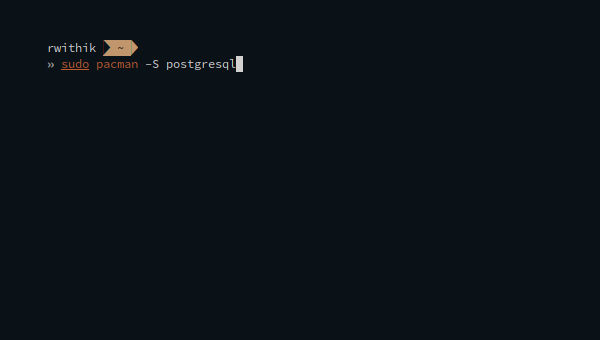
\includegraphics[width=\linewidth]{../Images/Installation/1.png}\newline
		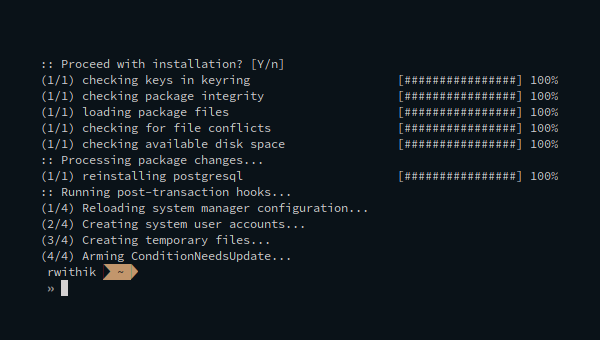
\includegraphics[width=\linewidth]{../Images/Installation/2.png}\newline
		\item You can switch to the PostgreSQL user by executing the following command:
		\begin{verbatim}
$ sudo -iu postgres
		\end{verbatim}
\end{enumerate}

\section{Initial Configuration}

\begin{enumerate}
	\item A database cluster must be initialized before \mintinline{psql}{postgres} can be used. Execute the following command as the postgres user:
	\begin{verbatim}
$ initdb -D /var/lib/postgres/data
	\end{verbatim}
	where -D option gives the location of the database cluster.
	Other optional arguments include:
		\begin{verbatim}
	    --locale=locale, where locale is to be chosen amongst the 
				system's available locales
		    -E encoding for the encoding (which must match the chosen locale);
		\end{verbatim}
		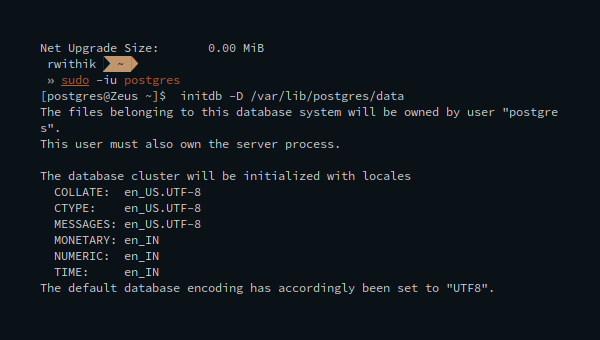
\includegraphics[width=\linewidth]{../Images/Installation/3.png}\newline
		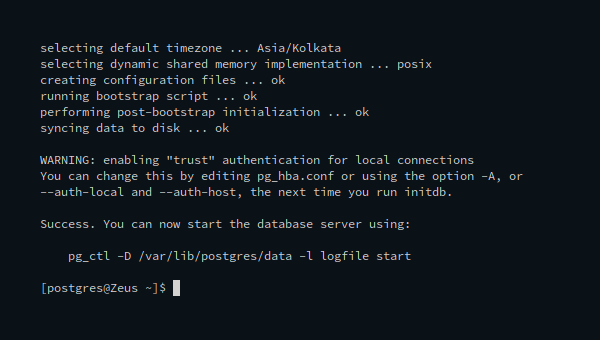
\includegraphics[width=\linewidth]{../Images/Installation/4.png}\newline
	\item Start and enable \verb-postgresql.service-. 
		\begin{verbatim}
		$ sudo systemctl start postgesql.service
		$ sudo systemtcl enable postgresql.service
		\end{verbatim}
		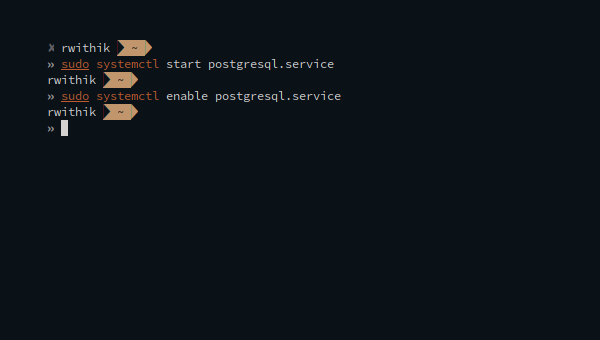
\includegraphics[width=\linewidth]{../Images/Installation/5.png}\newline
	\item Create a new database user. Execute this command as the \verb-postgres- user:
			\begin{verbatim}
			$ createuser --interactive
			\end{verbatim}
	\item Create a new database. Run this command as the regular user:
			\begin{verbatim}
			$ createdb myDatabaseName
			\end{verbatim}
		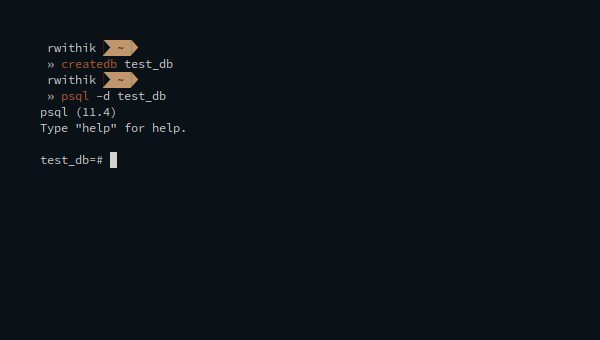
\includegraphics[width=\linewidth]{../Images/Installation/6.png}\newline
				
\end{enumerate}


}
\end{document}

\newpage

\chapter{Introduction to SQL}
\input{./53_Rwithik_Manoj_Introduction_to_Sql.tex}
\newpage

\chapter{Basic SQL Queries I}
\section{Aim}
 To study some basic SQL queries like, SELECT, INSERT, UPDATE, DELETE, and the WHERE clause.

\section{{Theory}}

\begin{itemize}
\item SELECT: Used to display the rows of a table. 
\item INSERT: Used to insert values into the table.
\item UPDATE: Used to update the values already inserted into the table based on the WHERE clause.
\item DELETE: Used to delete entries already inserted into the table based on the WHERE clause.
\item WHERE clause: Used to check for the presence or absence of a condition. 
\end{itemize}

\section{{Code and Output}}

\begin{enumerate}
\item Display the details of all the employees.\newline
\begin{minted}{sql}

SELECT * FROM employee

\end{minted}
\newline
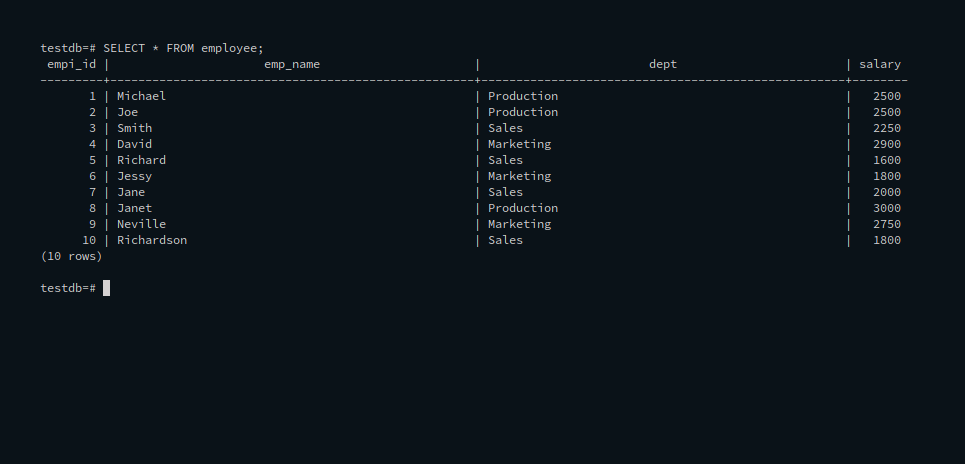
\includegraphics[width=\linewidth]{../Images/Basics/1.png}\newline
\item Display the names and id’s of all employees.\newline
\begin{minted}{sql}

SELECT emp_id, emp_name FROM employee;

\end{minted}
\newline
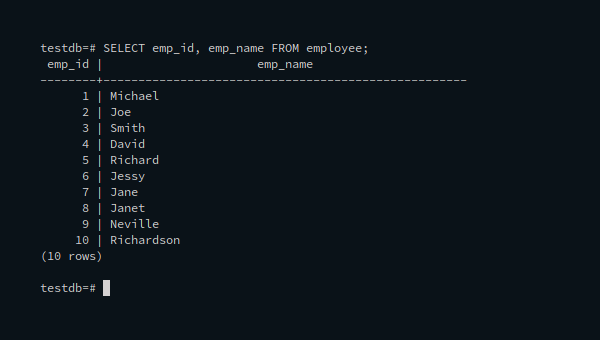
\includegraphics[width=\linewidth]{../Images/Basics/2.png}\newline
\item Delete the entry corresponding to employee id:10.\newline
\begin{minted}{sql}

DELETE FROM employee WHERE emp_id=10;

\end{minted}
\newline
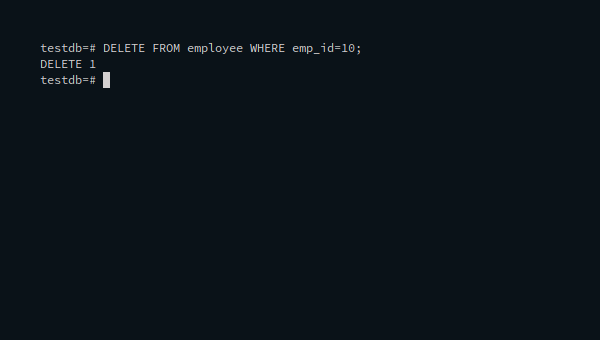
\includegraphics[width=\linewidth]{../Images/Basics/3.png}\newline
\item Insert a new tuple to the table. The salary field of the new employee should be kept NULL.\newline
\begin{minted}{sql}

INSERT INTO employee (emp_id, emp_name, dept) 
	VALUES (11, 'John', 'Sales');

\end{minted}
\newline
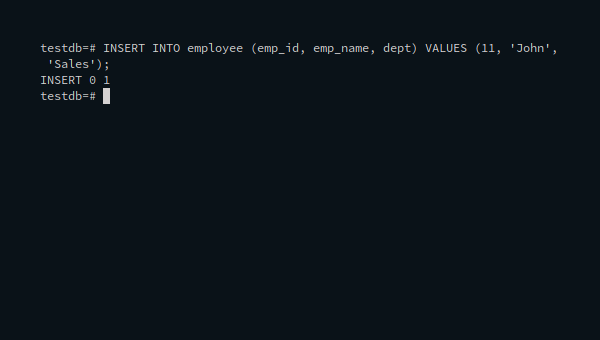
\includegraphics[width=\linewidth]{../Images/Basics/4.png}\newline
\item Find the details of all employees working in the marketing department.\newline
\begin{minted}{sql}

SELECT * FROM employee WHERE dept='Marketing';

\end{minted}
\newline
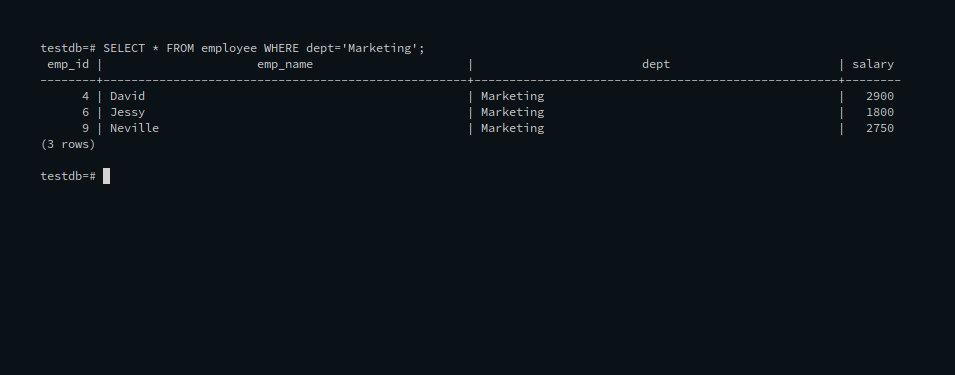
\includegraphics[width=\linewidth]{../Images/Basics/5.png}\newline
\item Add the salary details of the newly added employee.\newline
\begin{minted}{sql}

UPDATE employee SET salary = 1900 WHERE emp_id=10;

\end{minted}
\newline
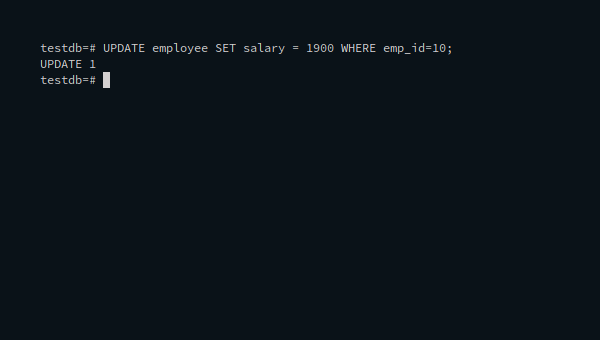
\includegraphics[width=\linewidth]{../Images/Basics/6.png}\newline
\item Update the salary of Richard to 1900\$.\newline
\begin{minted}{sql}

UPDATE employee SET salary = 1900 
	WHERE emp_name='Richard';

\end{minted}
\newline
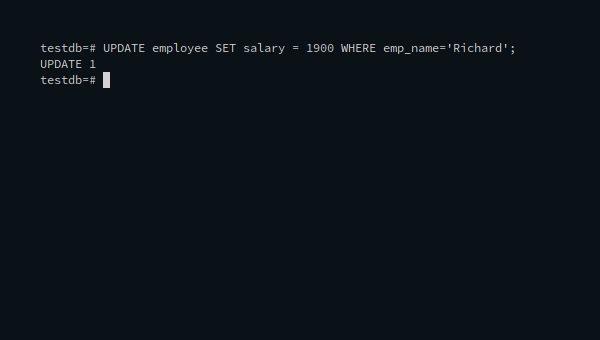
\includegraphics[width=\linewidth]{../Images/Basics/7.png}\newline
\item Find the details of all employees who are working for marketing and has a salary greater than	2000\$.\newline
\begin{minted}{sql}

SELECT * FROM employee 
	WHERE dept='Marketing' AND salary > 2000;

\end{minted}
\newline
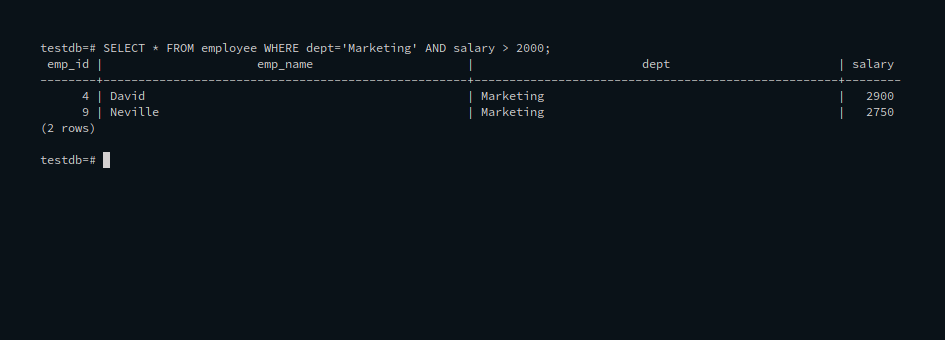
\includegraphics[width=\linewidth]{../Images/Basics/8.png}\newline
\item List the names of all employees working in the sales department and marketing department.\newline
\begin{minted}{sql}

SELECT emp_name FROM employee 
	WHERE dept='Sales' OR dept='Marketing';

\end{minted}
\newline
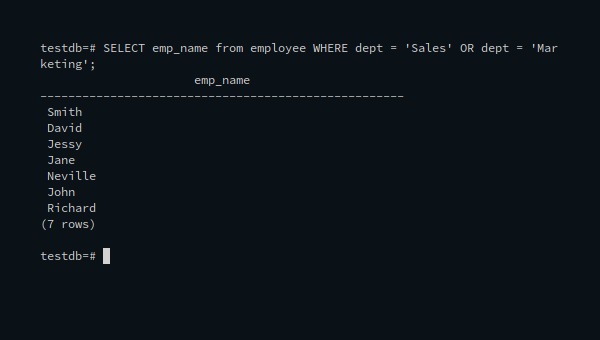
\includegraphics[width=\linewidth]{../Images/Basics/9.png}\newline
\item List the names and department of all employees whose salary is between2300\$ and 3000\$.\newline
\begin{minted}{sql}

SELECT emp_name FROM employee 
	WHERE salary BETWEEN 2300 AND 3000;

\end{minted}
\newline
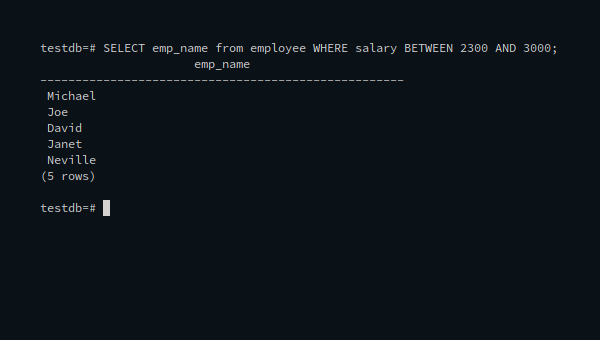
\includegraphics[width=\linewidth]{../Images/Basics/10.png}\newline
\item Update the salary of all employees working in production department 12\%.\newline
\begin{minted}{sql}

UPDATE employee SET salary = salary*1.12 
	WHERE dept='Production';
\end{minted}
\newline
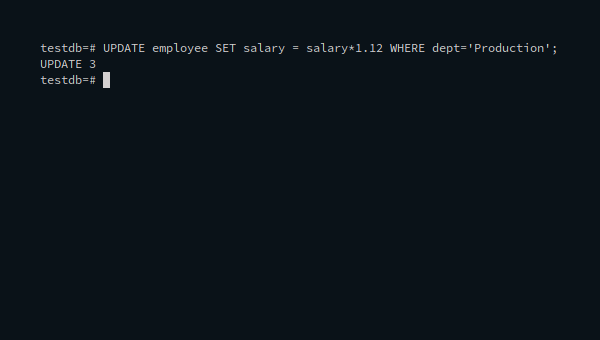
\includegraphics[width=\linewidth]{../Images/Basics/11.png}\newline
\item Display the names of all employees whose salary is less than 2000\$ or working for sales department.\newline
\begin{minted}{sql}

SELECT * FROM employee 
	WHERE salary < 2000 OR dept = 'Sales';

\end{minted}
\newline
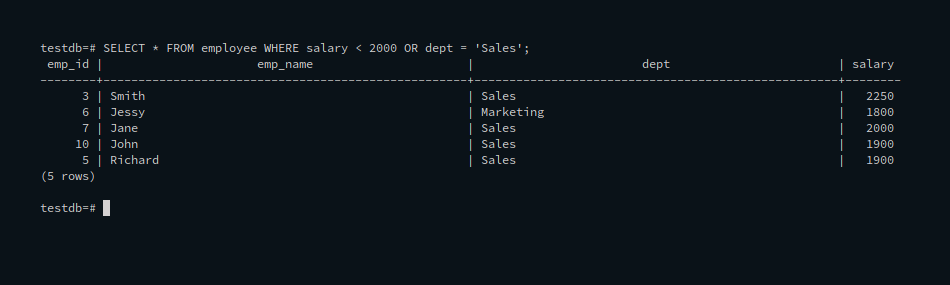
\includegraphics[width=\linewidth]{../Images/Basics/12.png}\newline
\end{enumerate}

\section{Result}
Implemented the program for Basic SQL Queries using Postgresql 11.5 on Manjaro Linux and the output was obtained.
\newpage

\chapter{Basic SQL Queries II}
\documentclass[10pt,a4paper,titlepage]{report}
\usepackage[utf8]{inputenc}
\usepackage{amsmath}
\usepackage{amsfonts}
\usepackage{amssymb}
\usepackage{graphicx}
\usepackage{xcolor}
\usepackage{minted}

\newcommand{\HRule}[1]{\rule{\linewidth}{#1}}

\nonstopmode


\begin{document}
{\fontfamily{cmr}\selectfont
\title{ \normalsize \textsc{}
\\ [2.0cm]
\HRule{0.5pt} \\
\LARGE \textbf{\uppercase{basic sql queries ii}
\HRule{2pt} \\ [0.5cm]
\normalsize \today \vspace*{5\baselineskip}}
}

\date{}

\author{
	Rwithik Manoj \\
	College of Engineering, Trivandrum \\
	Department of Computer Science and Engineering }

\maketitle
\newpage

\sectionfont{\scshape}

\begin{enumerate}
	\item List the names of all companies as mentioned in the database\newline
		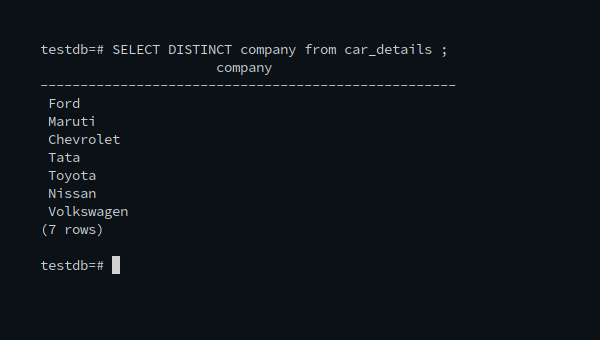
\includegraphics[width=\linewidth]{../Images/Basics/13.png}\newline
	\item List the names of all countries having car production companies\newline
		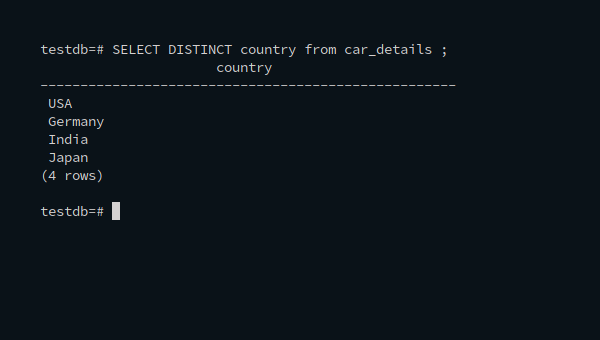
\includegraphics[width=\linewidth]{../Images/Basics/14.png}\newline
	\item List the details of all cars within a price range 4 to 7 lakhs\newline
		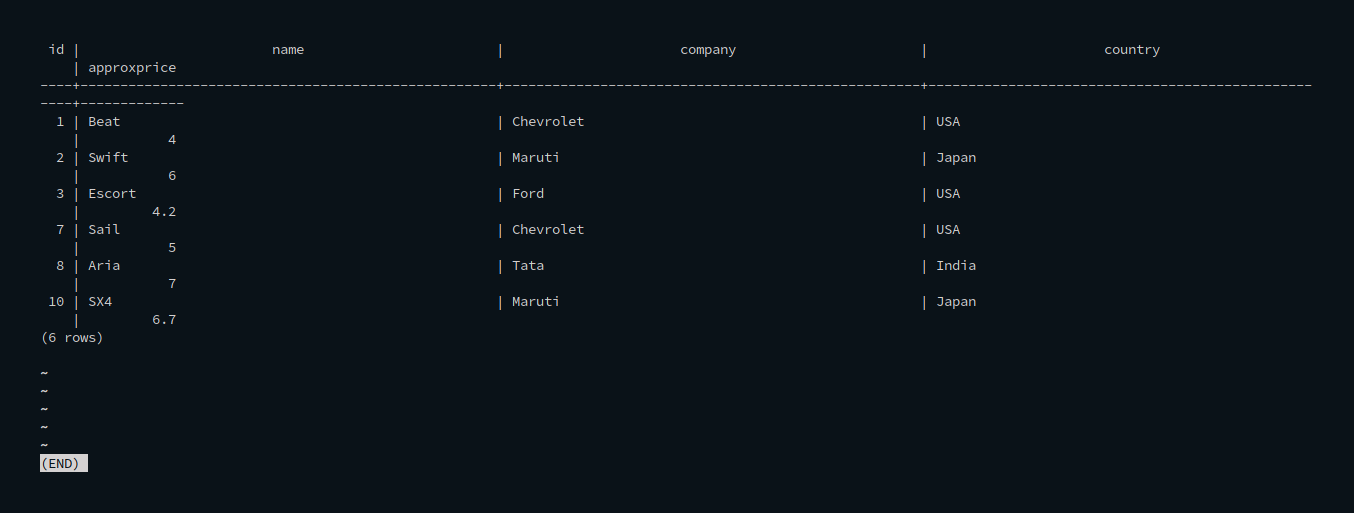
\includegraphics[width=\linewidth]{../Images/Basics/15.png}\newline
	\item List the name and company of all cars originating from Japan and having price less than 6 lakhs\newline
		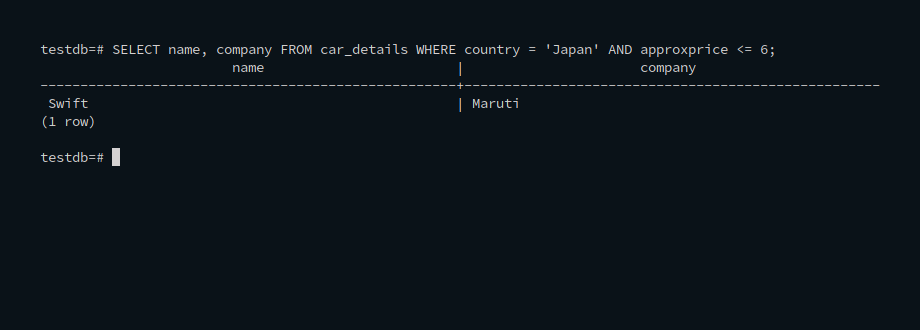
\includegraphics[width=\linewidth]{../Images/Basics/16.png}\newline
	\item List the names and the companies of all cars either from Nissan or having a price greater than 20 lakhs.\newline
		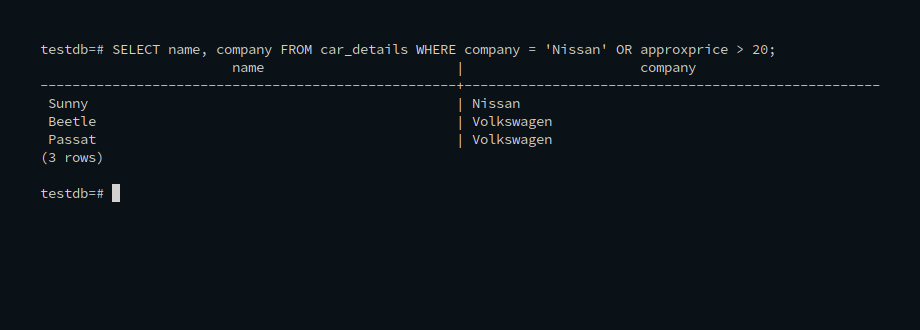
\includegraphics[width=\linewidth]{../Images/Basics/17.png}\newline
\item List the names of all cars produced by (Maruti,Ford).Use SQL IN statement.\newline
		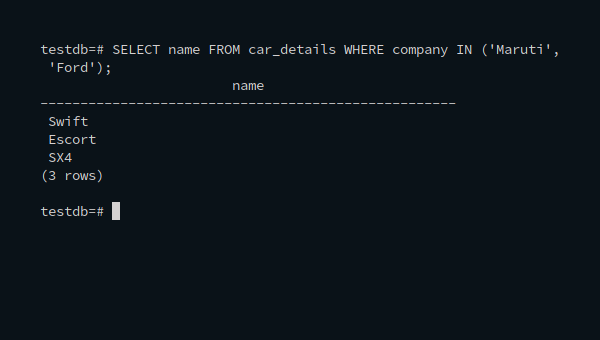
\includegraphics[width=\linewidth]{../Images/Basics/18.png}\newline
\item Alter the table cars to add a new field year (model release year).Upadate the year column for all the rows in the database.\newline
		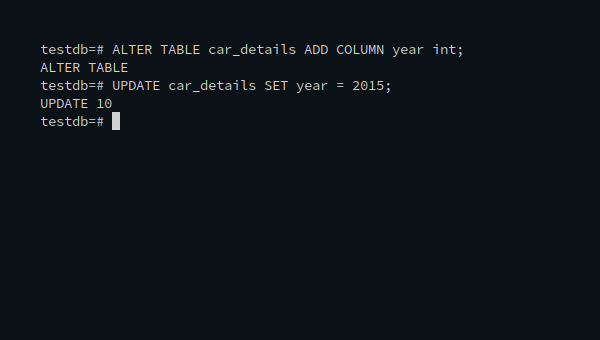
\includegraphics[width=\linewidth]{../Images/Basics/19.png}\newline
\item Display the names of all cars as Car\_name (while displaying the name attribute should be listed as car\_aliases)\newline
		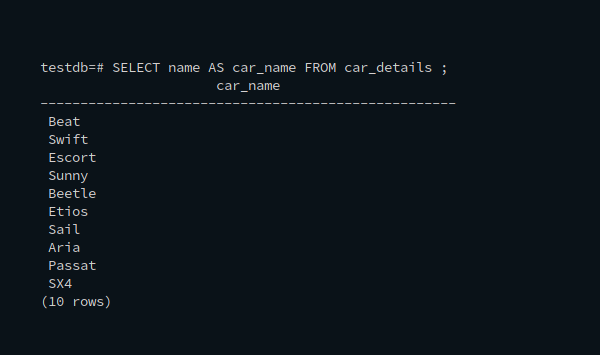
\includegraphics[width=\linewidth]{../Images/Basics/20.png}\newline
	\item Rename the attribute name to car\_name\newline
		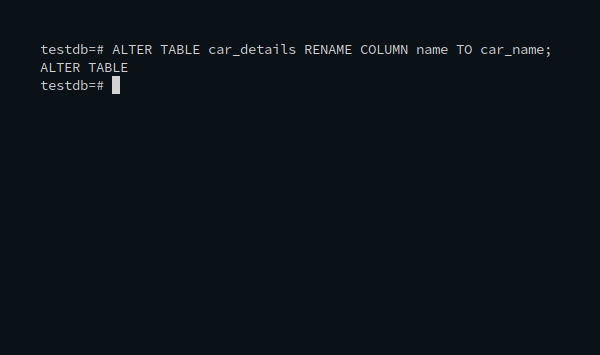
\includegraphics[width=\linewidth]{../Images/Basics/21.png}\newline
\item List the car manufactured by Toyota(to be displayed as cars\_Toyota)\newline
		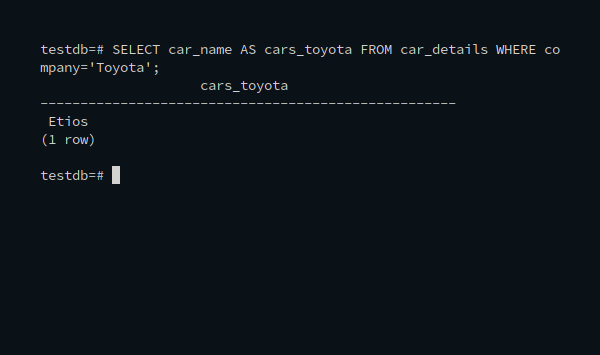
\includegraphics[width=\linewidth]{../Images/Basics/22.png}\newline
	\item List the details of all cars in alphabetical order\newline
		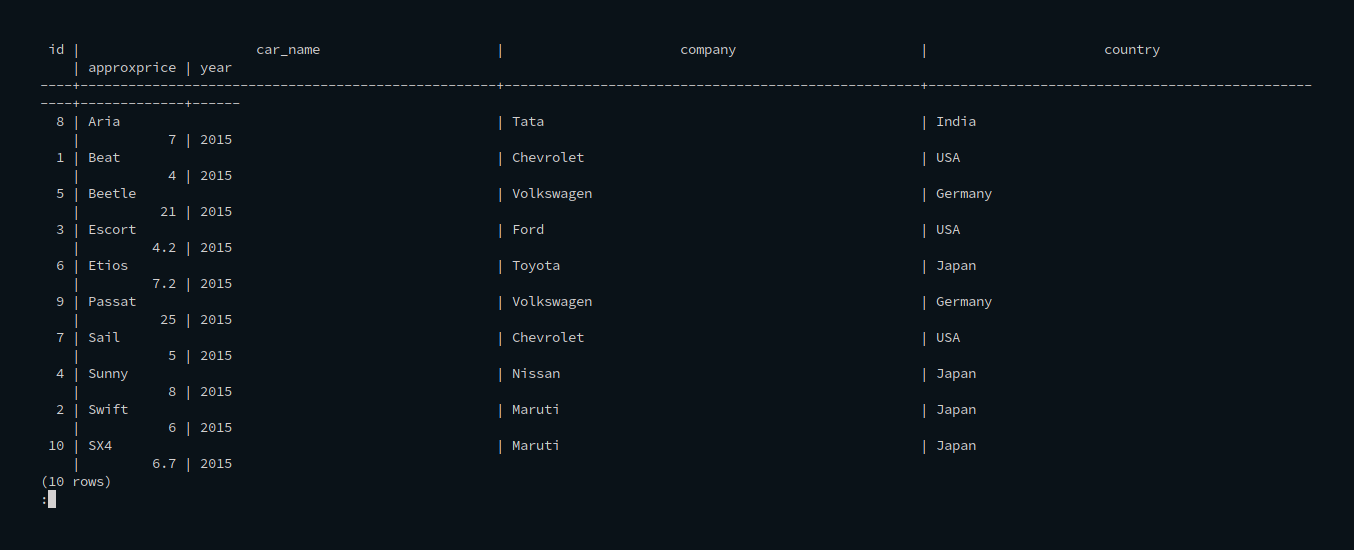
\includegraphics[width=\linewidth]{../Images/Basics/23.png}\newline
	\item List the details of all cars from cheapest to costliest.\newline
		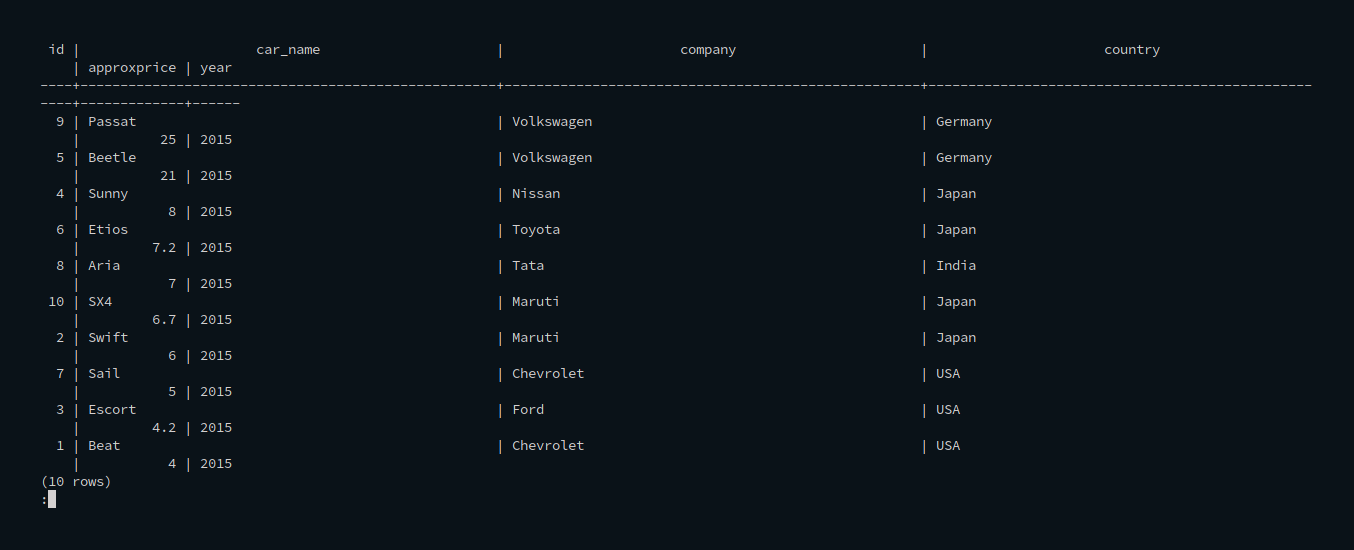
\includegraphics[width=\linewidth]{../Images/Basics/24.png}\newline
\end{enumerate}

\subsubsection{RESULT}

The query was executed successfully and output was verified.

}
\end{document}

\newpage

\chapter{Aggregate Functions}
\section{Aim}
 To study aggregate function: SUM, COUNT, AVG, MAX, MIN.

\section{{Theory}}

The Aggregate Functions in SQL are: 
\begin{itemize}
	\item SUM(): Used to find the sum of the values over a column
	\item MIN(): Used to find the minimum value in a column.
	\item MAX(): Used to find the maximum value in a column.
	\item AVG(): Used to find the average over a column.
	\item COUNT(): Used to count the number of rows in the output.
\end{itemize}

\section{{Code and Output}}

\begin{enumerate}
\item Find the class average for the subject ‘Physics’\newline
\begin{minted}{sql}

SELECT AVG(physics) FROM students;

\end{minted}
\newline
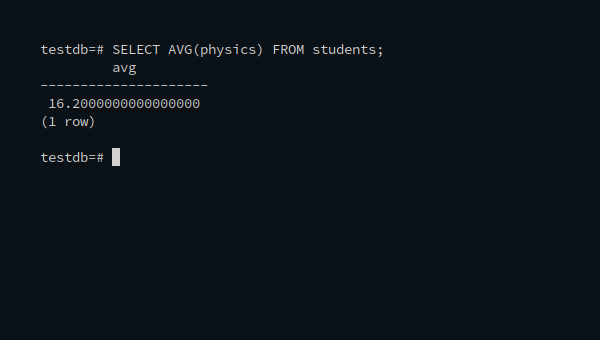
\includegraphics[width=\linewidth]{../Images/Aggregate/1.png}\newline
\item Find the highest marks for mathematics (To be displayed as highest\_marks\_maths).\newline
\begin{minted}{sql}

SELECT MAX(maths) AS highest_marks_maths FROM students;

\end{minted}
\newline
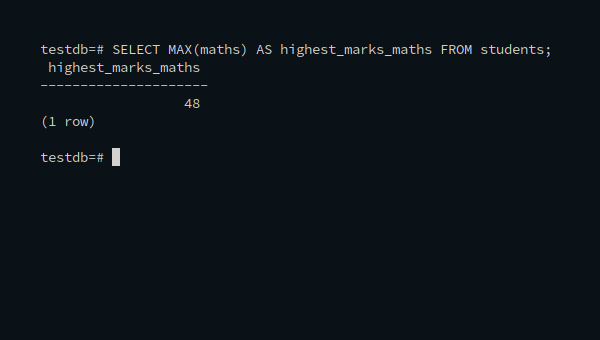
\includegraphics[width=\linewidth]{../Images/Aggregate/2.png}\newline
\item Find the lowest marks for chemistry(To be displayed as lowest\_mark\_chemistry)\newline
\begin{minted}{sql}

SELECT MIN(chemistry) AS lowest_marks_chemistry 
	FROM students;

\end{minted}
\newline
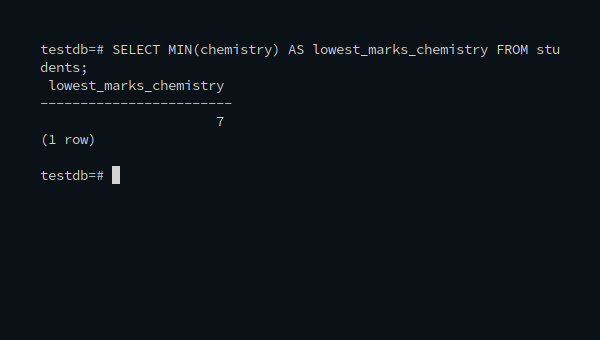
\includegraphics[width=\linewidth]{../Images/Aggregate/3.png}\newline
\item Find the total number of students who has got a ‘pass’ in physics.\newline
\begin{minted}{sql}

SELECT COUNT(*) AS passed_physics FROM students 
	WHERE physics > 12;

\end{minted}
\newline
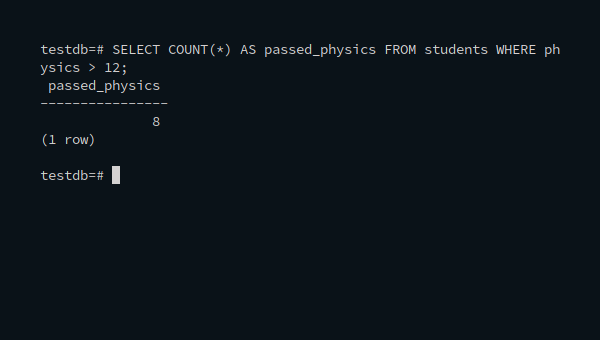
\includegraphics[width=\linewidth]{../Images/Aggregate/4.png}\newline
\item Generate the list of students who have passed in all the subjects\newline
\begin{minted}{sql}

SELECT * FROM students 
	WHERE physics > 12 AND chemistry > 12 AND maths > 25;

\end{minted}
\newline
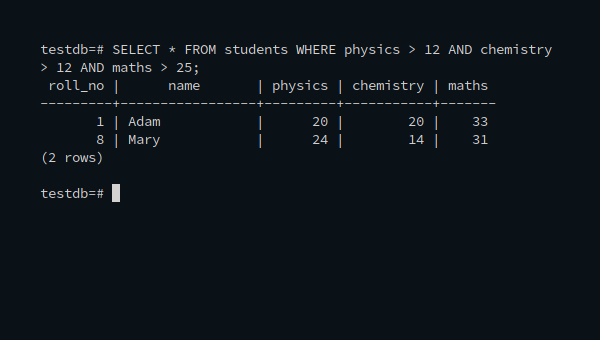
\includegraphics[width=\linewidth]{../Images/Aggregate/5.png}\newline
\item Generate a rank list for the class.Indicate Pass/Fail. Ranking based on total marks obtained by the
students.\newline
\begin{minted}{sql}

ALTER TABLE students ADD COLUMN result CHAR(1);
UPDATE students SET result = 'P' 
	WHERE physics > 12 AND chemistry > 12 AND maths > 25
UPDATE students SET result = 'F' 
	WHERE physics < 12 OR chemistry < 12 OR maths < 25
UPDATE students 
	SET total_marks = chemistry+physics+maths;
SELECT * FROM students ORDER BY total_marks;

\end{minted}
\newline
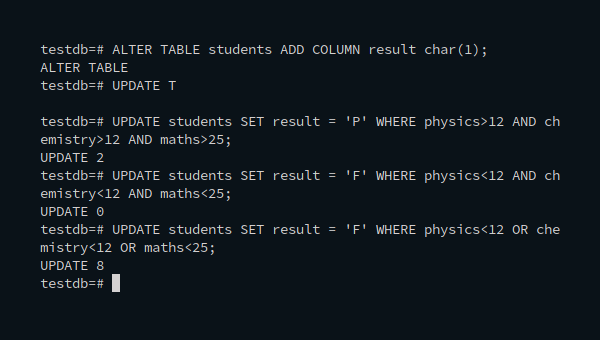
\includegraphics[width=\linewidth]{../Images/Aggregate/6.png}
\newline
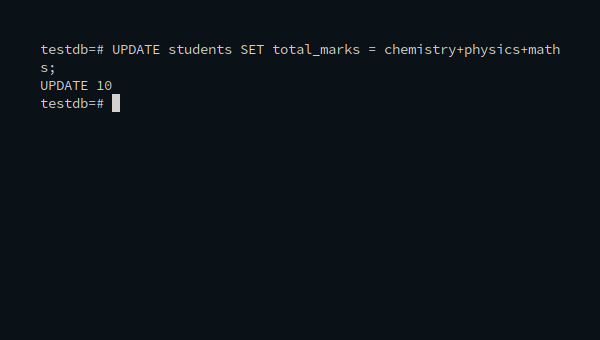
\includegraphics[width=\linewidth]{../Images/Aggregate/7.png}
\newline
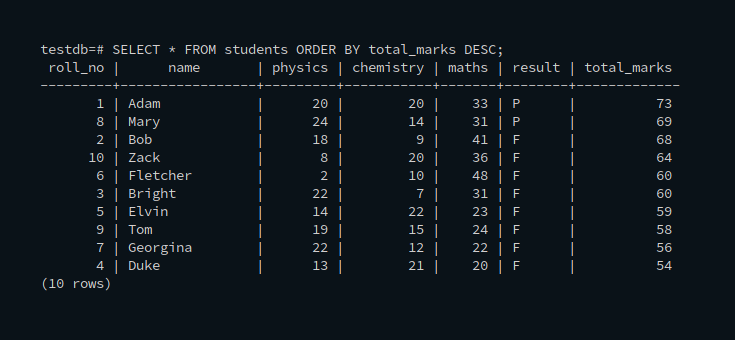
\includegraphics[width=\linewidth]{../Images/Aggregate/8.png}\newline
\item Find pass percentage of the class for mathematics.\newline
\begin{minted}{sql}

SELECT COUNT(*) * 100 / (SELECT COUNT(*) FROM students) 
	AS pass_perc_maths FROM students WHERE maths > 25;

\end{minted}
\newline
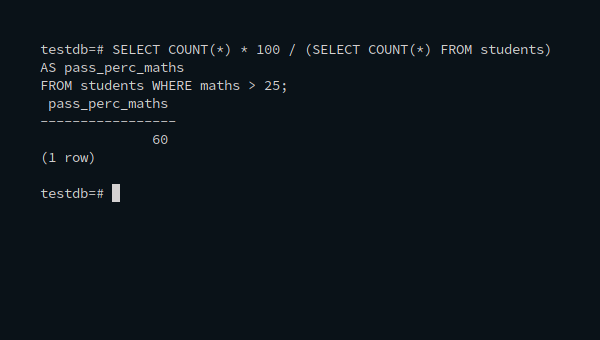
\includegraphics[width=\linewidth]{../Images/Aggregate/10.png}\newline
\item Find the overall pass percentage for all class.\newline
\begin{minted}{sql}

SELECT COUNT(*) * 100 / (SELECT COUNT(*) FROM students) 
	AS pass_perc FROM students 
	WHERE maths > 25 AND physics > 12 and chemistry > 12;

\end{minted}
\newline
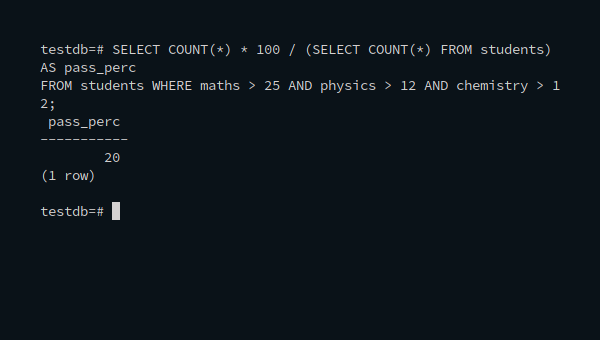
\includegraphics[width=\linewidth]{../Images/Aggregate/11.png}\newline
\item Find the class average.\newline
\begin{minted}{sql}

SELECT AVG(total_marks) FROM students;

\end{minted}
\newline
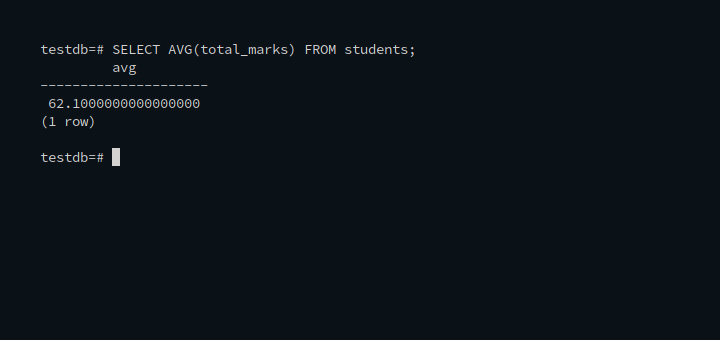
\includegraphics[width=\linewidth]{../Images/Aggregate/12.png}\newline
\item Find the total number of students who have got a Pass.\newline
\begin{minted}{sql}

SELECT COUNT(*) FROM students WHERE result = 'P';

\end{minted}
\newline
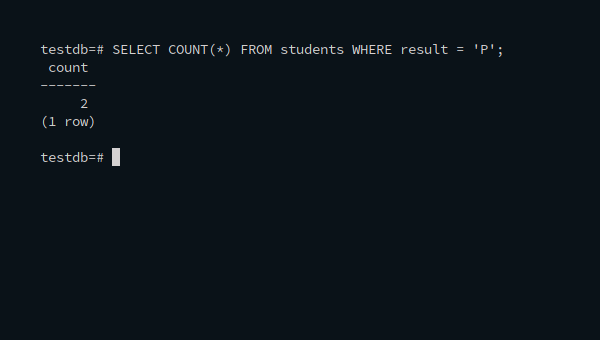
\includegraphics[width=\linewidth]{../Images/Aggregate/13.png}\newline
\end{enumerate}

\section{Result}
Implemented the program for Aggregate Functions using Postgresql 11.5 on Manjaro Linux and the output was obtained.
\newpage

\chapter{Data Constraints and Views}
\section{Aim}
 To study about various data constraints and views in SQL.

\section{{Theory}}

\subsection{Data Constraints}

The following are commonly used constraints available in PostgreSQL.
\begin{itemize}
    \item NOT NULL Constraint - Ensures that a column cannot have NULL value.
    \item UNIQUE Constraint - Ensures that all values in a column are different.
    \item PRIMARY Key - Uniquely identifies each row/record in a database table.
    \item FOREIGN Key - Constrains data based on columns in other tables.
    \item CHECK Constraint - The CHECK constraint ensures that all values in a column satisfy certain conditions.
\end{itemize}

\subsection{Views}

Views are pseudo-tables. That is, they are not real tables, but they appear as ordinary tables to SELECT. A view can represent a subset of a real table, selecting certain columns or certain rows from an ordinary table. A view can even represent joined tables. Because views are assigned separate permissions, you can use them to restrict table access so that the users see only specific rows or columns of a table.

\subsubsection{Syntax}

\begin{minted}{sql}
CREATE [TEMP | TEMPORARY] VIEW view_name AS
SELECT column1, column2.....
FROM table_name
WHERE [condition];
\end{minted}

\section{{Code and Output}}

\begin{enumerate}
\item
\begin{enumerate}
\item Create a table named Subjects with the given attributes
\begin{itemize}
\item Subid( Should not be NULL)
\item Subname (Should not be NULL)
\end{itemize}
Populate the database. Make sure that all constraints are working properly.\newline
\begin{minted}{sql}

CREATE TABLE subjects(
	subid int not null,
	subname char(20) not null
	);

INSERT INTO subjects VALUES(1, 'Maths');
INSERT INTO subjects VALUES(1, 'Physics');
INSERT INTO subjects VALUES(1, 'Chemistry');
INSERT INTO subjects VALUES(1, 'English');


\end{minted}
\newline
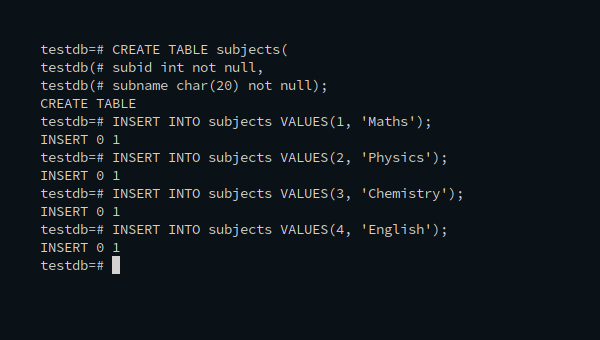
\includegraphics[width=\linewidth]{../Images/Constraints/1.png}\newline
\begin{enumerate}
\item Alter the table to set subid as the primary key.\newline
\begin{minted}{sql}

ALTER TABLE subjects ADD CONSTRAINT 
	pk PRIMARY KEY(subid);

\end{minted}
\newline
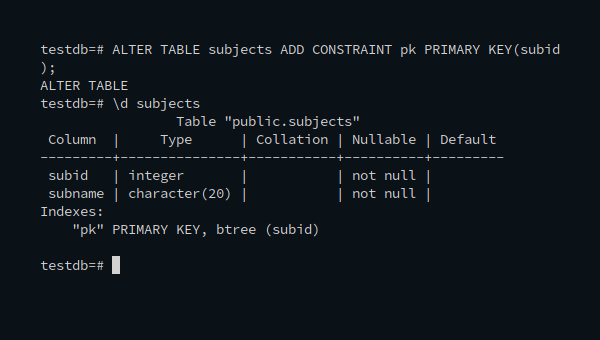
\includegraphics[width=\linewidth]{../Images/Constraints/2.png}\newline
\end{enumerate}
\item Create a table named Staff with the given attributes:
\begin{itemize}
\item staffid (Should be UNIQUE)
\item staffname
\item dept
\item age (Greater than 22)
\item salary (Less than 35000)
\end{itemize}
Populate the database. Make sure that all constraints are working properly.\newline
\begin{minted}{sql}

CREATE TABLE staff(
	staffid int unique,
	staffname char(20),
	delt char(15),
	age int check(age > 22),
	salary int check(salary < 35000)
	);
INSERT INTO staff 
	VALUES(1, 'John', 'Purchasing', 24, 30000);

INSERT INTO staff 
	VALUES(2, 'Sera', 'Sales', 25, 20000);
	
INSERT INTO staff 
	VALUES(3, 'John', 'Sales', 28, 25000);

\end{minted}
\newline
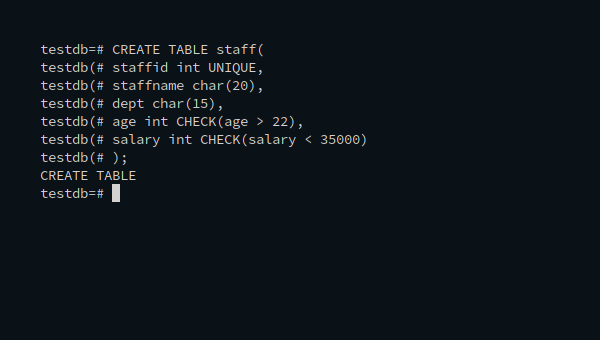
\includegraphics[width=\linewidth]{../Images/Constraints/3.png}\newline
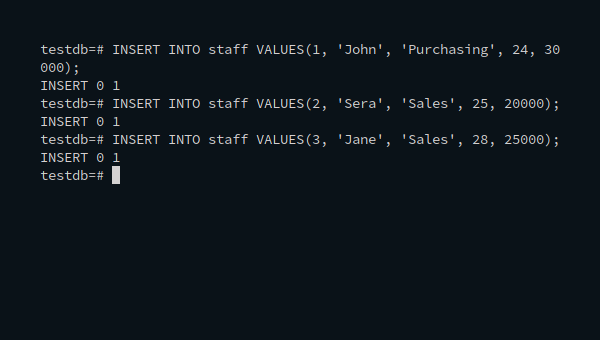
\includegraphics[width=\linewidth]{../Images/Constraints/4.png}\newline
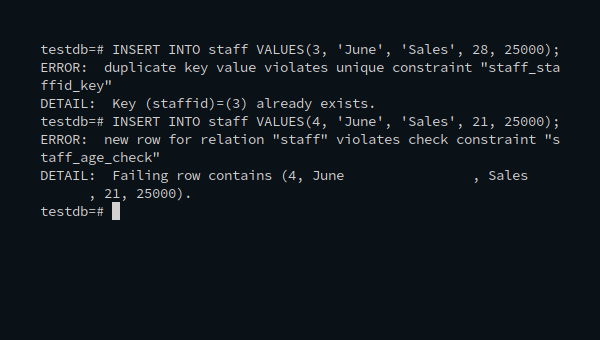
\includegraphics[width=\linewidth]{../Images/Constraints/5.png}\newline
\begin{enumerate}
\item Delete the check constraint imposed on the attribute salary\newline
\begin{minted}{sql}

ALTER TABLE staff 
	DROP CONSTRAINT staff_salary_check;

\end{minted}
\newline
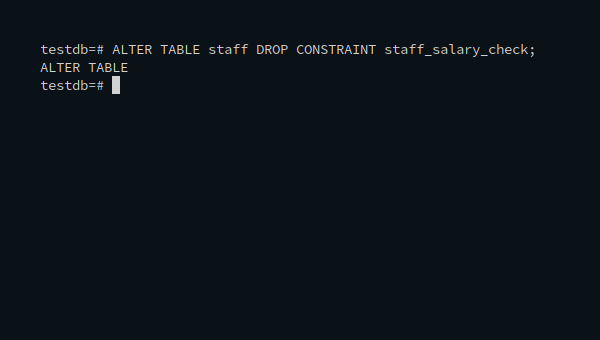
\includegraphics[width=\linewidth]{../Images/Constraints/6.png}\newline
\item Delete the unique constraint on the attribute staffid\newline
\begin{minted}{sql}

ALTER TABLE staff 
	DROP CONSTRAINT staff_salary_key;

\end{minted}
\newline
\includegraphics[width=\linewidth]{../Images/Constraints/7.png}\newline
\end{enumerate}
\item Create a table named Bank with the following attributes
\begin{itemize}
\item bankcode (To be set as Primary Key, type= varchar(3) )
\item bankname (Should not be NULL)
\item headoffice
\item branches (Integer value greater than Zero)
\end{itemize}
Populate the database. Make sure that all constraints are working properly.All constraints have to be set after creating the table.\newline
\begin{minted}{sql}

CREATE TABLE bank(
	bankcode varchar(3),
	bankname varchar(10),
	headoffice varchar(10),
	branches int
	);
ALTER TABLE bank 
	ADD CONSTRAINT bank_pk PRIMARY KEY(bankcode),
	ADD CONSTRAINT bnk_bankname_not_null 
		CHECK bankname IS NOT NULL),
	ADD CONSTRAINT bank_branches_check 
		CHECK(branches > 0);

\end{minted}
\newline
\includegraphics[width=\linewidth]{../Images/Constraints/8.png}\newline
\newline
\includegraphics[width=\linewidth]{../Images/Constraints/9.png}\newline
\newline
\includegraphics[width=\linewidth]{../Images/Constraints/10.png}\newline
\item Create a table named Branch with the following attributes
\begin{itemize}
\item branchid (To be set as Primary Key)
\item branchname (Set Default value as ‘New Delhi’)
\item bankid (Foreign Key:- Refers to bank code of Bank table)
\end{itemize}
\begin{enumerate}
\item Populate the database. Make sure that all constraints are working properly.\newline
\begin{minted}{sql}

CREATEA TABLE branch(
	branchid PRIMARY KEY,
	branchname varchar(10) DEFAULT 'New Delhi',
	bankid varchar(10) 
		REFERENCES bank(bankcode)
		ON DELETE CASCADE
	);

\end{minted}
\newline
\includegraphics[width=\linewidth]{../Images/Constraints/11.png}\newline
\item During database population, demonstrate how the DEFAULT Constraint is satisfied.\newline
\begin{minted}{sql}

INSERT INTO branch(branchid, bankid) VALUES (02, 'AAA');

\end{minted}
\newline
\includegraphics[width=\linewidth]{../Images/Constraints/12.png}\newline
\item Delete the bank with bank code ‘SBT’ and make sure that the corresponding entries are getting deleted from the related tables.\newline
\begin{minted}{sql}

DELETE FROM bank WHERE bankcode = 'SBT';

\end{minted}
\newline
\includegraphics[width=\linewidth]{../Images/Constraints/13.png}\newline
\item Drop the Primary Key using ALTER command\newline
\begin{minted}{sql}

ALTER TABLE branch DROP CONSTRAINT branch_pkey;

\end{minted}
\newline
\includegraphics[width=\linewidth]{../Images/Constraints/14.png}\newline
\end{enumerate}
\end{enumerate}
\item Create a View named sales\_staff to hold the details of all staff working in sales Department\newline
\begin{minted}{sql}

CREATE VIEW sales_dept AS
	SELECT * FROM staff WHERE dept='Sales';

\end{minted}
\newline
\includegraphics[width=\linewidth]{../Images/Constraints/15.png}\newline

\item Drop table branch. Create another table named branch and name all the constraints as given below:
\begin{itemize}
\item Constraint name Column Constraint
\item Pk branch\_id Primary key
\item Df branch\_name Default :’New Delhi’
\item Fk bankid Foreign key/References
\end{itemize}
\begin{minted}{sql}

DROP TABLE branch;
CREATE TABLE branch(
	branchid int,
	branchname varchar(10),
	bankid varchar(3)
	);
ALTER TABLE branch
	ADD CONSTRAINT Pk PRIMARY KEY(branchid),
	ADD CONSTRAINT Fk FOREIGN KEY(bankid) 
		REFERENCES bank(bankcode)
ALTER TABLE branch ALTER COLUMN branchname 
	SET DEFAULT 'New Delhi';

\end{minted}
\newline
\includegraphics[width=\linewidth]{../Images/Constraints/16.png}\newline
\begin{enumerate}
\item Delete the default constraint in the table\newline
\begin{minted}{sql}

ALTER TABLE branch ALTER COLUMN branchname DROP DEFAULT;

\end{minted}
\newline
\includegraphics[width=\linewidth]{../Images/Constraints/17.png}\newline
\item Delete the primary key constraint\newline
\begin{minted}{sql}

ALTER TABLE branch DROP CONSTRAINT Pk;

\end{minted}
\newline
\includegraphics[width=\linewidth]{../Images/Constraints/18.png}\newline
\end{enumerate}

\item Update the view sales\_staff to include the details of staff belonging to sales department whose salary is greater than 20000.\newline
\begin{minted}{sql}

INSERT INTO staff VALUES(3, 'Jane', 'Sales', 28, 25000);

\end{minted}
\newline
\includegraphics[width=\linewidth]{../Images/Constraints/19.png}\newline
\item Delete the view sales\_staff.\newline
\begin{minted}{sql}

DROP VIEW sales_dept;

\end{minted}
\newline
\includegraphics[width=\linewidth]{../Images/Constraints/20.png}\newline

\end{enumerate}



\section{Result}
Implemented the program for Data Constraints and Views using Postgresql 11.5 on Manjaro Linux and the output was obtained.
\newpage

\chapter{String Functions and Pattern Matching}
\section{Aim}
 To study string functions like, UPPER, LOWER, REVERSE, LPAD, LTRIM, RPAD, RTRIM, the LIKE keyword, and the wildcard characters.

\section{{Theory}}

\subsection{String Functions}
\begin{itemize}
	\item UPPER(str): Converts str to upper case.
	\item LOWER(str): Converts str to lower case.
	\item REVERSE(str): Reverses str.
	\item LPAD(str, len, padstr): Left pads the string to length len with the padding string padstr.
	\item RPAD(str, len, padstr): Right pads the string to length len with the padding string padstr.
	\item LTRIM(str, charset): Removes the characters from charset, from the left end of the string.
	\item RTRIM(str, charset): Removes the characters from charset, from the right end of the string.
	\item INITCAP(str): Changes the first letter of each word to its capital letter.
	\item CONCAT(str1, str2): Concatenates str2 to str1.
	\item LENGTH(str): Returns the length of the string str.
	\item SUBSTR(str, startindex, endindex): Returns the substring of str from startindex to endindex
\end{itemize}

\section{LIKE keyword}

The like keyword is used to match certain patterns in the strings. It is usually used in conjunction with two wildcard characters:
\begin{enumerate}
	\item \% character: This character matches zero or more occurances of any character\newline
	For example, 'A\%' can match any string starting with 'A'.
	\item \_ character: This character matches exactly one occurance of any character.\newline
	For example, 'A\_\_\_\_' matches any string starting with A, of length 5.
\end{enumerate}

\section{{Code and Output}}

\subsubsection{Create a table named acct\_details and populate the table as shown below.}

\newline
\includegraphics[width=\linewidth]{../Images/Strings/1.png}

\begin{enumerate}
\item Find the names of all people starting on the alphabet 'D'.\newline
\begin{minted}{sql}

SELECT name FROM acct_details WHERE name LIKE 'D%';

\end{minted}
\newline
\includegraphics[width=\linewidth]{../Images/Strings/2.png}
\item List the names of all branches containing the substring 'New'.\newline
\begin{minted}{sql}

SELECT branch FROM acct_details WHERE branch LIKE '%New%';

\end{minted}
\newline
\includegraphics[width=\linewidth]{../Images/Strings/3.png}
\item List all the names in Upper Case Format.\newline
\begin{minted}{sql}

SELECT UPPER(name) FROM acct_details;

\end{minted}
\newline
\includegraphics[width=\linewidth]{../Images/Strings/4.png}
\item List the names where the 4th letter is 'n' and last letter is 'n'.\newline
\begin{minted}{sql}

SELECT name FROM actt_details WHERE name LIKE '___n%n';

\end{minted}
\newline
\includegraphics[width=\linewidth]{../Images/Strings/5.png}
\item List the names starting on 'D' , 3rd letter is 'a' and contains the substring 'Eli'.\newline
\begin{minted}{sql}

SELECT name FROM acct_details WHERE 
	name LIKE '%D_a%' AND LIKE '%Eli%';

\end{minted}
\newline
\includegraphics[width=\linewidth]{../Images/Strings/6.png}
\item List the names of people whose account number ends in '6'.\newline
\begin{minted}{sql}

SELECT name FROM acct_details WHERE acct_no LIKE '%6';

\end{minted}
\newline
\includegraphics[width=\linewidth]{../Images/Strings/7.png}
\item Update the table so that all the names are in Upper Case Format.\newline
\begin{minted}{sql}

UPDATE acct_details SET name=UPPER(name);

\end{minted}
\newline
\includegraphics[width=\linewidth]{../Images/Strings/8.png}
\item List the names of all people ending on the alphabet 't'.\newline
\begin{minted}{sql}

SELECT name FROM acct_details WHERE name LIKE '%T';

\end{minted}
\newline
\includegraphics[width=\linewidth]{../Images/Strings/9.png}
\item List all the names in reverse.\newline
\begin{minted}{sql}

SELECT REVERSE(name) FROM acct_details;

\end{minted}
\newline
\includegraphics[width=\linewidth]{../Images/Strings/10.png}
\item Display all the phone numbers including US Country code ( +1). For eg: (378)400-1234 should be displayed as +1(378)400-1234. Use LPAD function.\newline
\begin{minted}{sql}

SELECT LPAD(phone, 16, '+1') FROM acct_details;

\end{minted}
\newline
\includegraphics[width=\linewidth]{../Images/Strings/11.png}
\item Display all the account numbers. The starting alphabet associated with the Account\_No should be removed. Use LTRIM function.\newline
\begin{minted}{sql}

SELECT LTRIM(acct_no, '[ABCD]') AS acc_no, 
	branch, name, phone FROM acct_details;

\end{minted}
\newline
\includegraphics[width=\linewidth]{../Images/Strings/12.png}
\item Display the details of all people whose account number starts in '4' and name contains the substring 'Williams'.\newline
\begin{minted}{sql}

SELECT * FROM acct_details WHERE 
	acct_no LIKE '_4%' AND name LIKE '%WILLIAMS%';

SELECT * FROM acct_details WHERE 
	acct_no LIKE '_5%' AND name LIKE '%WILLIAMS%';

\end{minted}
\newline
\includegraphics[width=\linewidth]{../Images/Strings/13.png}
\end{enumerate}

\subsubsection{String Functions}

\begin{enumerate}
\item Find the reverse of the string 'nmutuAotedOehT'.\newline
\begin{minted}{sql}

SELECT REVERSE('nmutuAotedOehT')

\end{minted}
\newline
\includegraphics[width=\linewidth]{../Images/Strings/14.png}
\item Use LTRIM function on '123231xyzTech' so as to obtain the output 'Tech'.\newline
\begin{minted}{sql}

SELECT LTRIM('123231xyzTech', '123XYZ');

\end{minted}
\newline
\includegraphics[width=\linewidth]{../Images/Strings/15.png}
\item Use RTRIM function on 'Computer ' to remove the trailing spaces.\newline
\begin{minted}{sql}

SELECT RTRIM('COMPUTER      ');

\end{minted}
\newline
\includegraphics[width=\linewidth]{../Images/Strings/16.png}
\item Perform RPAD on 'computer' to obtain the output as 'computerXXXX'.\newline
\begin{minted}{sql}

SELECT RPAD('COMPUTER', 12, 'X');

\end{minted}
\newline
\includegraphics[width=\linewidth]{../Images/Strings/17.png}
\item Perform INITCAP function on 'mARK cALAwaY'.\newline
\begin{minted}{sql}

SELECT INITCAP('mARK cALAwaY')

\end{minted}
\newline
\includegraphics[width=\linewidth]{../Images/Strings/18.png}
\item Find the length of the string 'Database Management Systems'.\newline
\begin{minted}{sql}

SELECT LENGTH('Database Management Systems');

\end{minted}
\newline
\includegraphics[width=\linewidth]{../Images/Strings/19.png}
\item Concatenate the strings 'Julius' and 'Caesar'\newline
\begin{minted}{sql}

SELECT CONCAT('Julius', 'Caesar');

\end{minted}
\newline
\includegraphics[width=\linewidth]{../Images/Strings/20.png}
\item Use SUBSTR function to retrieve the substring 'is' from the string 'India is my country'.\newline
\begin{minted}{sql}

SELECT SUBSTR('India is my country', 7, 2);

\end{minted}
\newline
\includegraphics[width=\linewidth]{../Images/Strings/21.png}
\end{enumerate}

\section{Result}
Implemented the program for String Functions and Pattern Matching using Postgresql 11.5 on Manjaro Linux and the output was obtained.
\newpage

\chapter{Join Statements, Set Operations, Nested Queries and Grouping}
\documentclass[10pt,a4paper,titlepage]{report}
\usepackage[utf8]{inputenc}
\usepackage{amsmath}
\usepackage{amsfonts}
\usepackage{amssymb}
\usepackage{graphicx}
\usepackage{xcolor}
\usepackage{minted}

\newcommand{\HRule}[1]{\rule{\linewidth}{#1}}

\nonstopmode


\begin{document}
{\fontfamily{cmr}\selectfont
\title{ \normalsize \textsc{}
\\ [2.0cm]
\HRule{0.5pt} \\
\LARGE \textbf{\uppercase{JOIN STATEMENTS, SET OPERATIONS, NESTED QUERIES AND
GROUPING}
\HRule{2pt} \\ [0.5cm]
\normalsize August 13, 2019 \vspace*{5\baselineskip}}
}

\date{}

\author{
	Rwithik Manoj \\
	College of Engineering, Trivandrum \\
	Department of Computer Science and Engineering }

\maketitle
\newpage

\sectionfont{\scshape}

\subsection*{Tables and their schemas}

\subsubsection{Items}
itemid (primary key) 
itemname 
category
price
instock

\subsubsection{Customers}
custid (primary key)
custname
address
state

\subsubsection{Orders}
orderid (primary key)
itemid
quantity
orderdate

\subsubsection{Delivery}
delivery id (primary key)
custid
orderid

\includegraphics[width=\linewidth]{../Images/Joins/tables.png}

\subsection{Questions}

\begin{enumerate}
	\item List the details of all customers who have placed an order\newline
	\includegraphics[width=\linewidth]{../Images/Joins/1.png}
	\item List the details of all customers whose orders have been delivered\newline
	\includegraphics[width=\linewidth]{../Images/Joins/2.png}
	\item Find the orderdate for all customers whose name starts in the letter ‘J’\newline
	\includegraphics[width=\linewidth]{../Images/Joins/3.png}
	\item Display the name and price of all items bought by the customer ‘Mickey’\newline
	\includegraphics[width=\linewidth]{../Images/Joins/4.png}
	\item List the details of all customers who have placed an order after January 2013 and not received delivery of items.\newline
	\includegraphics[width=\linewidth]{../Images/Joins/5.png}
	\item Find the itemid of items which has either been ordered or not delivered. (Use UNION)\newline
	\includegraphics[width=\linewidth]{../Images/Joins/6.png}
	\item Find the name of all customers who have placed an order and have their orders delivered.(Use SET INTERSECTION)\newline
	\includegraphics[width=\linewidth]{../Images/Joins/7.png}
	\item Find the custname of all customers who have placed an order but not having their ordersdelivered. (Use SET MINUS)\newline
	\includegraphics[width=\linewidth]{../Images/Joins/8.png}
	\item Find the name of the customer who has placed the most number of orders.\newline
	\includegraphics[width=\linewidth]{../Images/Joins/9.png}
	\item Find the details of all customers who have purchased items exceeding a price of 5000\$.\newline
	\includegraphics[width=\linewidth]{../Images/Joins/10.png}
	\item Find the name and address of customers who has not ordered a 'Samsung Galaxy S4'\newline
	\includegraphics[width=\linewidth]{../Images/Joins/11.png}
	\item Perform Left Outer Join and Right Outer Join on Customers & Orders Table.\newline
	\includegraphics[width=\linewidth]{../Images/Joins/12.png}
	\item Find the details of all customers grouped by state.\newline
	\includegraphics[width=\linewidth]{../Images/Joins/13.png}
	\item Display the details of all items grouped by category and having a price greater than the average price of all items.\newline
	\includegraphics[width=\linewidth]{../Images/Joins/14.png}
\end{enumerate}

\subsubsection*{RESULT}
The query was executed and output was successfully obtained.

}
\end{document}

\newpage

\chapter{PL/SQL and Sequence}
\documentclass[10pt,a4paper,titlepage]{report}
\usepackage[utf8]{inputenc}
\usepackage{amsmath}
\usepackage{amsfonts}
\usepackage{amssymb}
\usepackage{graphicx}
\usepackage{xcolor}
\usepackage{minted}

\newcommand{\HRule}[1]{\rule{\linewidth}{#1}}

\nonstopmode


\begin{document}
{\fontfamily{cmr}\selectfont
\title{ \normalsize \textsc{}
\\ [2.0cm]
\HRule{0.5pt} \\
\LARGE \textbf{\uppercase{PL/SQL AND SEQUENCE}
\HRule{2pt} \\ [0.5cm]
\normalsize \today \vspace*{5\baselineskip}}
}

\date{}

\author{
	Rwithik Manoj \\
	College of Engineering, Trivandrum \\
	Department of Computer Science and Engineering }

\maketitle
\newpage

\sectionfont{\scshape}

\begin{enumerate}
	\item To print the first ‘n’ prime numbers.\newline
	\begin{verbatim}
	CREATE OR REPLACE FUNCTION primes(n INTEGER)
		RETURNS INTEGER AS
	$$
	DECLARE
		counter INTEGER := 0;
		i INTEGER := 2;
		prime_list TEXT;
		divisors INTEGER := 0;
	BEGIN
		WHILE counter < n LOOP
			FOR j IN 2..i/2 LOOP
				IF (i%j = 0) THEN
					divisors := divisors + 1;
				END IF;
			END LOOP;
			IF (divisors = 0) THEN
				RAISE NOTICE '%', i;
				counter := counter + 1;
			END IF;
			divisors := 0;
			i := i + 1;
		END LOOP;
		RETURN NULL;
	END;
	$$ LANGUAGE plpgsql;
	\end{verbatim}
	\includegraphics[width=\linewidth]{../Images/Plsql/1.png}

	\item Display the Fibonacci series upto ‘n’ terms.\newline
	\begin{verbatim}
	CREATE OR REPLACE FUNCTION fibonacci (n INTEGER)
	   RETURNS INTEGER AS $$
	DECLARE
	   i INTEGER := 0 ;
	   j INTEGER := 1 ;
	BEGIN

	   IF (n < 1) THEN
	      RETURN null ;
	   END IF;

	   LOOP
	      EXIT WHEN i > n ;
				raise notice '%', i;
	      SELECT j, i + j INTO i,   j ;
	   END LOOP ;

		 RETURN null;
	END ;
	$$ LANGUAGE plpgsql;
	\end{verbatim}
	\includegraphics[width=\linewidth]{../Images/Plsql/2.png}

	\item Create a table named student\_grade with the given attributes: roll, name, mark1, mark2, mark3, grade. Calculate the grade of the student and insert a it into the table using PL/SQL. ( Grade= 'PASS' if AVG greater than 40, Grade ='FAIL' otherwise.)\newline
	\begin{verbatim}
	CREATE OR REPLACE FUNCTION marks()
	RETURNS INTEGER
	AS $$
	DECLARE
		total INTEGER := 0;
	BEGIN
		UPDATE student_marks SET grade='PASS' WHERE (mark1 + mark2 + mark3) / 3 > 40;
	  UPDATE student_marks SET grade='FAIL' WHERE (mark1 + mark2 + mark3) / 3 <= 40;
		RETURN null;
	END;
	$$ LANGUAGE plpgsql;

	\end{verbatim}
	\includegraphics[width=\linewidth]{../Images/Plsql/3.png}

	\item Create table circle\_area (rad,area). For radius 5, 10, 15, 20 and 25, find the area and insert the corresponding values into the table by using loop structure in PL/SQL.\newline
	\begin{verbatim}
	CREATE OR REPLACE FUNCTION area()
	RETURNS TABLE(r REAL, area REAL)
	AS $$
	BEGIN

		FOR r IN 1..5 LOOP
			INSERT INTO circles VALUES(5*r, 22*5*r/7);
		END LOOP;
		RETURN QUERY SELECT * FROM circles;
	END;
	$$ LANGUAGE plpgsql;
	\end{verbatim}
	\includegraphics[width=\linewidth]{../Images/Plsql/4.png}

	\item Use an array to store the names and marks of 10 students in a class. Using loop structures in PL/SQL insert the ten tuples to a table named stud. \newline
	\begin{verbatim}
	CREATE OR REPLACE FUNCTION students_data_entry()
	RETURNS INTEGER
	AS $$
	DECLARE
		names TEXT ARRAY := '{"ARUN", "AMAL", "PETER", "JOSE", "ANNIE", "MARY", "JOSEPH", "MARK", "MIDHUN", "KEVIN"}';
		marks INTEGER ARRAY := '{25, 76, 43, 45, 67, 57, 97, 56, 89, 8}';
	BEGIN
		FOR i IN 1..10 LOOP
			INSERT INTO students_data VALUES (names[i], marks[i]);
		END LOOP;
		RETURN null;
	END;
	$$ LANGUAGE plpgsql;

	\end{verbatim}
	\includegraphics[width=\linewidth]{../Images/Plsql/5.png}

	\item Create a sequence using PL/SQL. Use this sequence to generate the primary key values for a table named class\_cse with attributes roll, name and phone\_no. Insert some tuples using PL/SQL programming.\newline
	\begin{verbatim}
	CREATE OR REPLACE FUNCTION generate_data()
	RETURNS INTEGER
	AS $$
	BEGIN
		CREATE SEQUENCE numbers;
		INSERT INTO class_cse VALUES(nextval('numbers'), 'ARUN', '0482-239091');
		INSERT INTO class_cse VALUES(nextval('numbers'), 'AMAL', '0484-234562');
		INSERT INTO class_cse VALUES(nextval('numbers'), 'PETER', '0485-11234');
		INSERT INTO class_cse VALUES(nextval('numbers'), 'JOSE', '0481-43617');
		DROP SEQUENCE numbers;
		RETURN null;
	END;
	$$ LANGUAGE plpgsql;
	\end{verbatim}
	\includegraphics[width=\linewidth]{../Images/Plsql/6.png}

\end{enumerate}

\subsubsection{RESULT}
The PL/SQL programs were executed successfully and the output was obtained.

}
\end{document}

\newpage

\chapter{Cursors}
\documentclass[10pt,a4paper,titlepage]{report}
\usepackage[utf8]{inputenc}
\usepackage{amsmath}
\usepackage{amsfonts}
\usepackage{amssymb}
\usepackage{graphicx}
\usepackage{xcolor}
\usepackage{minted}

\newcommand{\HRule}[1]{\rule{\linewidth}{#1}}

\nonstopmode


\begin{document}
{\fontfamily{cmr}\selectfont
\title{ \normalsize \textsc{}
\\ [2.0cm]
\HRule{0.5pt} \\
\LARGE \textbf{\uppercase{Cursors}
\HRule{2pt} \\ [0.5cm]
\normalsize \today \vspace*{5\baselineskip}}
}

\date{}

\author{
	Rwithik Manoj \\
	College of Engineering, Trivandrum \\
	Department of Computer Science and Engineering }

\maketitle
\newpage

\sectionfont{\scshape}

\begin{enumerate}
		\item Create table student (id, name, m1, m2, m3, grade). Insert 5 tuples into it. Find the total, calculate grade and update the grade in the table.
	\begin{verbatim}

CREATE OR REPLACE FUNCTION grader()
RETURNS INTEGER
AS $$
DECLARE
	cur CURSOR FOR SELECT * FROM student;
	rec RECORD;
	total INTEGER;
	grd CHAR(1);
BEGIN
	OPEN cur;
	LOOP
		total := 0;
		FETCH cur into rec;
		EXIT WHEN NOT FOUND;
		total := rec.m1 + rec.m2 + rec.m3;
		IF total > 250 THEN
			grd := 'A';
		ELSIF total > 200 THEN
			grd := 'B';
		ELSIF total > 150 THEN
			grd := 'C';
		ELSIF total > 100 THEN
			grd := 'D';
		ELSE
			grd := 'F';
		END IF;
		UPDATE student SET grade = grd WHERE CURRENT OF cur;
	END LOOP;
	CLOSE cur;
	RETURN null;
END;
$$ LANGUAGE plpgsql;
	\end{verbatim}
	\includegraphics[width=\linewidth]{../Images/Cursors/1.png}

	\item Create bank\_details (accno, name, balance, adate).Calculate the interest of the amount and insert into a new table with fields (accno, interest). Interest = 0.08 * balance.\newline
	\includegraphics[width=\linewidth]{../Images/Cursors/2.png}
	\begin{verbatim}
	
CREATE OR REPLACE FUNCTION interest()
RETURNS INTEGER
AS $$
DECLARE
	cur CURSOR FOR SELECT * FROM bank_details;
	rec RECORD;
	intr REAL;
BEGIN
	CREATE TABLE bank_new(acc_no int, interest real);
	OPEN cur;
	LOOP
		FETCH cur into rec;
		EXIT WHEN NOT FOUND;
		intr := rec.balance * 0.08;
		INSERT INTO bank_new VALUES(rec.accno, intr);
	END LOOP;
	CLOSE cur;
	RETURN null;
END;
$$ LANGUAGE plpgsql;
	\end{verbatim}

	\item Create table people\_list (id, name, dt\_joining, place).If person’s experience is above 10 years, put the tuple in table exp\_list (id, name, experience).\newline
	\begin{verbatim}

CREATE OR REPLACE FUNCTION exp()
RETURNS INTEGER
AS $$
DECLARE
	cur CURSOR FOR SELECT * FROM people_list;
	rec RECORD;
BEGIN
	OPEN cur;
	LOOP
		FETCH cur into rec;
		EXIT WHEN NOT FOUND;
		IF rec.dt_joining < '2009-08-18' THEN
			INSERT INTO exp_list VALUES(rec.id, rec.name, ('2019-08-18' - rec.dt_joining)/365);
		END IF;
	END LOOP;
	CLOSE cur;
	RETURN null;
END;
$$ LANGUAGE plpgsql;
	\end{verbatim}
	\includegraphics[width=\linewidth]{../Images/Cursors/3.png}
\item Create table
employee\_list(id,name,monthly salary). If:\newline
  annual salary less than 60000, increment monthly salary by 25\% \newline
  between 60000 and 200000, increment by 20\%\newline
  between 200000 and 500000, increment by 15\%\newline
  annual salary greater than 500000, increment monthly salary by 10\%\newline
	\begin{verbatim}

CREATE OR REPLACE FUNCTION sal()
RETURNS INTEGER
AS $$
DECLARE
	cur CURSOR FOR SELECT * FROM employee_list;
	rec RECORD;
BEGIN
	OPEN cur;
	LOOP
		FETCH cur into rec;
		EXIT WHEN NOT FOUND;
		IF (rec.salary * 12) < 60000 THEN
			UPDATE employee_list SET salary = salary * 1.25 WHERE CURRENT OF cur;
		ELSIF (rec.salary * 12) < 200000 THEN
			UPDATE employee_list SET salary = salary * 1.2 WHERE CURRENT OF cur;
		ELSIF (rec.salary * 12) < 500000 THEN
			UPDATE employee_list SET salary = salary * 1.15 WHERE CURRENT OF cur;
		ELSE
			UPDATE employee_list SET salary = salary * 1.1 WHERE CURRENT OF cur;
		END IF;
	END LOOP;
	CLOSE cur;
	RETURN null;
END;
$$ LANGUAGE plpgsql;
	\end{verbatim}
	\includegraphics[width=\linewidth]{../Images/Cursors/4.png}

\end{enumerate}

\subsubsection{RESULT}
The PL/SQL programs were executed successfully and the output was obtained.

}
\end{document}

\newpage

\chapter{Triggers and Exception Handling}
\documentclass[10pt,a4paper,titlepage]{report}
\usepackage[utf8]{inputenc}
\usepackage{amsmath}
\usepackage{amsfonts}
\usepackage{amssymb}
\usepackage{graphicx}
\usepackage{xcolor}
\usepackage{minted}

\newcommand{\HRule}[1]{\rule{\linewidth}{#1}}

\nonstopmode


\begin{document}
{\fontfamily{cmr}\selectfont
\title{ \normalsize \textsc{}
\\ [2.0cm]
\HRule{0.5pt} \\
\LARGE \textbf{\uppercase{Triggers and Exceptions}
\HRule{2pt} \\ [0.5cm]
\normalsize \today \vspace*{5\baselineskip}}
}

\date{}

\author{
	Rwithik Manoj \\
	College of Engineering, Trivandrum \\
	Department of Computer Science and Engineering }

\maketitle
\newpage

\sectionfont{\scshape}

\subsubsection{Create a table customer\_details (cust\_id (unique), cust\_name, address).\newline
Create a table emp\_details(empid(unique), empname, salary).\newline
Create table cust\_count(count\_row).\newline
}
\begin{enumerate}
	\item Create a trigger whenever a new record is inserted in the customer\_details table.
	\begin{verbatim}

CREATE OR REPLACE FUNCTION log_last_name_changes()
  RETURNS trigger AS
$$
BEGIN
   RAISE NOTICE 'A new row was inserted';
	 RETURN NEW;
END;
$$ LANGUAGE plpgsql;

CREATE TRIGGER last_name_changes
  BEFORE INSERT
  ON customer_details
  FOR EACH ROW
  EXECUTE PROCEDURE log_last_name_changes();
	\end{verbatim}
	\includegraphics[width=\linewidth]{../Images/Triggers/1.png}

	\item Create a trigger to display a message when a user enters a value greater than 20000 in the salary field of emp\_details table.
	\begin{verbatim}

	CREATE OR REPLACE FUNCTION log_sal_changes()
	  RETURNS trigger AS
	$$
	BEGIN
		IF NEW.salary > 20000 THEN
	  	RAISE NOTICE 'Employee has salary greater than 20000/-';
		END IF;
		RETURN NEW;
	END;
	$$ LANGUAGE plpgsql;

	CREATE TRIGGER salary_changes
	  BEFORE INSERT
	  ON emp_details
	  FOR EACH ROW
	  EXECUTE PROCEDURE log_sal_changes();


	\end{verbatim}
	\includegraphics[width=\linewidth]{../Images/Triggers/2.png}

	\item Create a trigger w.r.t customer\_detailstable.Increment the value of count\_row (in cust\_count table) whenever a new tuple is inserted and decrement the value of count\_row when a tuple is deleted. Initial value of the count\_row is set to 0.
	\begin{verbatim}
	
CREATE OR REPLACE FUNCTION update_count()
	RETURNS trigger AS
$$
BEGIN
	UPDATE cust_count SET count_row = (SELECT count(*) FROM customer_details);
	RETURN NEW;
END;
$$ LANGUAGE plpgsql;

CREATE TRIGGER count_changes
	AFTER INSERT OR DELETE
	ON customer_details
	FOR EACH ROW
	EXECUTE PROCEDURE update_count();

	\end{verbatim}
	\includegraphics[width=\linewidth]{../Images/Triggers/3.png}
	\includegraphics[width=\linewidth]{../Images/Triggers/8.png}

	\item Create a trigger to insert the deleted rows from emp\_details to another table and updated rows to another table.(Create the tables deleted and updated)
	\begin{verbatim}
CREATE OR REPLACE FUNCTION archive_deleted()
	RETURNS trigger AS
$$
BEGIN
	INSERT INTO deleted VALUES(OLD.*);
	RETURN NEW;
END;
$$ LANGUAGE plpgsql;

CREATE OR REPLACE FUNCTION archive_updated()
	RETURNS trigger AS
$$
BEGIN
	INSERT INTO updated VALUES(OLD.*);
	RETURN NEW;
END;
$$ LANGUAGE plpgsql;

CREATE TRIGGER archive_deleted_trig
	BEFORE DELETE
	ON emp_details
	FOR EACH ROW
	EXECUTE PROCEDURE archive_deleted();

CREATE TRIGGER archive_updated_trig
	BEFORE UPDATE
	ON emp_details
	FOR EACH ROW
	EXECUTE PROCEDURE archive_updated();

	\end{verbatim}
	\includegraphics[width=\linewidth]{../Images/Triggers/4.png}

	\item Write a PL/SQL to show divide by zero exception
	\begin{verbatim}
CREATE OR REPLACE FUNCTION divide(a REAL, b REAL)
RETURNS REAL AS
$$
BEGIN
  IF b = 0 THEN
    RAISE EXCEPTION 'Division by Zero';
    RETURN null;
  ELSE
    RETURN a / b;
  END IF;
END;
$$ LANGUAGE plpgsql;

	\end{verbatim}
	\includegraphics[width=\linewidth]{../Images/Triggers/5.png}

	\item Write a PL/SQL to show no data found exception
	\begin{verbatim}
CREATE OR REPLACE FUNCTION func_ex() RETURNS trigger AS
$$
DECLARE
  var_name name;
BEGIN
WHEN NO_DATA_FOUND THEN RAISE EXCEPTION 'No data found. Try another query.';
RETURN NEW;
END;
$$ LANGUAGE plpgsql;
CREATE TRIGGER insert_trigger AFTER UPDATE ON people_list EXECUTE PROCEDURE func_ex();

	\end{verbatim}
	\includegraphics[width=\linewidth]{../Images/Triggers/6.png}


	\item Create a table with ebill(cname,prevreading,currreading). If prevreading = currreading then raise an exception ‘Data Entry Error’.
	\begin{verbatim}
CREATE OR REPLACE FUNCTION check_bill()
RETURNS TRIGGER AS
$$
BEGIN
  IF NEW.prevreading = NEW.currreading THEN
    RAISE EXCEPTION 'Data Entry Error';
    RETURN OLD;
  ELSE
    RETURN NEW;
  END IF;
END;
$$ LANGUAGE plpgsql;

CREATE TRIGGER bill_check
	BEFORE INSERT
	ON ebill
	FOR EACH ROW
	EXECUTE PROCEDURE check_bill();

\end{verbatim}

	\includegraphics[width=\linewidth]{../Images/Triggers/7.png}
\end{enumerate}

\subsubsection{RESULT}
The PL/SQL programs were executed successfully and the output was obtained.

}
\end{document}

\newpage

\chapter{Procedure, Functions and Packages}
\documentclass[10pt,a4paper,titlepage]{report}
\usepackage[utf8]{inputenc}
\usepackage{amsmath}
\usepackage{amsfonts}
\usepackage{amssymb}
\usepackage{graphicx}
\usepackage{xcolor}
\usepackage{minted}

\newcommand{\HRule}[1]{\rule{\linewidth}{#1}}

\nonstopmode


\begin{document}
{\fontfamily{cmr}\selectfont
\title{ \normalsize \textsc{}
\\ [2.0cm]
\HRule{0.5pt} \\
\LARGE \textbf{\uppercase{Functions and Procedures}
\HRule{2pt} \\ [0.5cm]
\normalsize \today \vspace*{5\baselineskip}}
}

\date{}

\author{
	Rwithik Manoj \\
	College of Engineering, Trivandrum \\
	Department of Computer Science and Engineering }

\maketitle
\newpage

\sectionfont{\scshape}

}
\begin{enumerate}
	\item Create a function factorial to find the factorial of a number. Use this function in a PL/pgSQL Program to display the factorial of a number.
	\begin{verbatim}
CREATE OR REPLACE FUNCTION factorial(n INTEGER)
RETURNS INTEGER AS
$$
DECLARE
	fact INTEGER := 1;
BEGIN
	IF n < 1 THEN
		RETURN 1;
	END IF;
	FOR i IN 1..n LOOP
		fact := fact * i;
	END LOOP;
	RAISE NOTICE 'Factorial is %', fact;
	RETURN fact;
END;
$$ LANGUAGE plpgsql;
	\end{verbatim}
	\includegraphics[width=\linewidth]{../Images/Functions/1.png}

	\item Create a table student\_details(roll int, marks int, phone int). Create a procedure pr1 toupdate all rows in the database. Boost the marks of all students by 5\%.
	\begin{verbatim}
CREATE OR REPLACE FUNCTION grading()
RETURNS INTEGER
AS $$
DECLARE
t INTEGER := 0
cur CURSOR FOR SELECT * FROM student
rec RECORD
grd CHAR(1)
BEGIN
OPEN cur
LOOP
t := 0
FETCH cur into rec
EXIT WHEN NOT FOUND
t := rec.m1 + rec.m2 + rec.m3
UPDATE student SET total = t WHERE CURRENT OF cur
IF t > 250 THEN
grd := 'A'
ELSIF t > 200 THEN
grd := 'B'
ELSIF t > 150 THEN
grd := 'C'
ELSIF t > 100 THEN
grd := 'D'
ELSE
grd := 'F'
END IF
CALL marks(rec.id, grd)
END LOOP
CLOSE cur
RETURN null
END
$$ LANGUAGE plpgsql

CREATE OR REPLACE PROCEDURE marks(tid INTEGER, tgrd CHAR)
LANGUAGE plpgsql
AS $$
BEGIN
UPDATE studentmark SET grade=tgrade WHERE id=tid
END
$$;
	\end{verbatim}
	\includegraphics[width=\linewidth]{../Images/Functions/2.png}

	\item Create table student (id, name, m1, m2, m3, total, grade).Create a function f1 to calculate grade. Create a procedure p1 to update the total and grade.\newline
Using a function to calculate the grade.\newline
Using a procedure to update the grade value for the tuple.\newline
	\begin{verbatim}
CREATE OR REPLACE FUNCTION grading()
RETURNS INTEGER
AS $$
DECLARE
	t INTEGER := 0;
	cur CURSOR FOR SELECT * FROM student;
	rec RECORD;
	grd CHAR(1);
BEGIN
	OPEN cur;
	LOOP
		t := 0;
		FETCH cur into rec;
		EXIT WHEN NOT FOUND;
		t := rec.m1 + rec.m2 + rec.m3;
		UPDATE student SET total = t WHERE CURRENT OF cur;
		IF t > 250 THEN
			grd := 'A';
		ELSIF t > 200 THEN
			grd := 'B';
		ELSIF t > 150 THEN
			grd := 'C';
		ELSIF t > 100 THEN
			grd := 'D';
		ELSE
			grd := 'F';
		END IF;
		CALL marks(rec.id, grd);
	END LOOP;
	CLOSE cur;
	RETURN null;
END;
$$ LANGUAGE plpgsql;
	\end{verbatim}
	\includegraphics[width=\linewidth]{../Images/Functions/3.png}

	\item Create a package pk1 consisting of the following functions and procedures 
	\begin{enumerate}
		\item Procedure proc1 to find the sum, average and product of two numbers 
		\item Procedure proc2 to find the square root of a number 
		\item Function named fn11 to check whether a number is even or not
		\item A function named fn22 to find the sum of 3 numbers 
	\end{enumerate}
		Use this package in a PL/SQL program. Call the functions f11, f22 and procedures pro1, pro2 within the program and display their results.
\end{enumerate}

\begin{verbatim}

CREATE SCHEMA pk1

CREATE OR REPLACE PROCEDURE pk1.proc1(num1 REAL,num2 REAL)
LANGUAGE plpgsql
AS
$$
DECLARE
sum REAL
average REAL
prod REAL
BEGIN
sum = num1 + num2
prod = num1 * num2
average = (num1 + num2) / 2
RAISE NOTICE 'Sum of % and % is %', num1, num2, sum
RAISE NOTICE 'Product of % and % is %', num1, num2, prod
RAISE NOTICE 'Average of % and % is %', num1, num2, average
END
$$

CREATE OR REPLACE PROCEDURE pk1.proc2(num1 REAL)
LANGUAGE plpgsql
AS
$$
DECLARE
root REAL
BEGIN
root = sqrt(num1)
RAISE NOTICE 'Root of % is %', num1, root
END
$$

CREATE OR REPLACE FUNCTION pk1.fn11(num REAL) RETURNS VOID AS
$$
DECLARE
rem INT 
BEGIN
rem = num
rem = rem %2
IF rem = 1 THEN
	RAISE NOTICE 'Number % is odd', num
	ELSE
		RAISE NOTICE 'Number % is even', num
		END IF
		END
		$$ LANGUAGE plpgsql

		CREATE OR REPLACE FUNCTION pk1.fn22(num1 REAL, num2 REAL, num3 REAL) RETURNS VOID AS
		$$
		DECLARE
		sum REAL 
		BEGIN
		sum = num1 + num2 + num3
		RAISE NOTICE 'Sum of % , %, % is %', num1, num2, num3, sum
		END
		$$ LANGUAGE plpgsql

		CREATE OR REPLACE FUNCTION pk1.all(num1 REAL, num2 REAL, num3 REAL)
		RETURNS VOID AS
		$$
		DECLARE
		BEGIN
		CALL pk1.proc1(num1, num2)
		CALL pk1.proc2(num1)
		PERFORM pk1.fn11(num1)
		PERFORM pk1.fn22(num1, num2, num3)
		END
		$$ LANGUAGE plpgsql;
\end{verbatim}

\includegraphics[width=\linewidth]{../Images/Functions/4.png}

\subsubsection{RESULT}
The PL/SQL programs were executed successfully and the output was obtained.

}
\end{document}

\newpage


    
}
\end{document}
